\section{RISC-V}

\begin{frame}{RISC-V}
    \begin{itemize}
        \item Libre y gratuita
        \item Conjunto de instrucciones reducido (RISC)
        \item Registro a Registro o load/store
        \item Modular
    \end{itemize}
    
    \nocite{RiscVSpec1}
    \nocite{RiscVExchangeCores}
\end{frame}

\begin{frame}{Familia SweRV}
    \begin{figure}
        \centering
        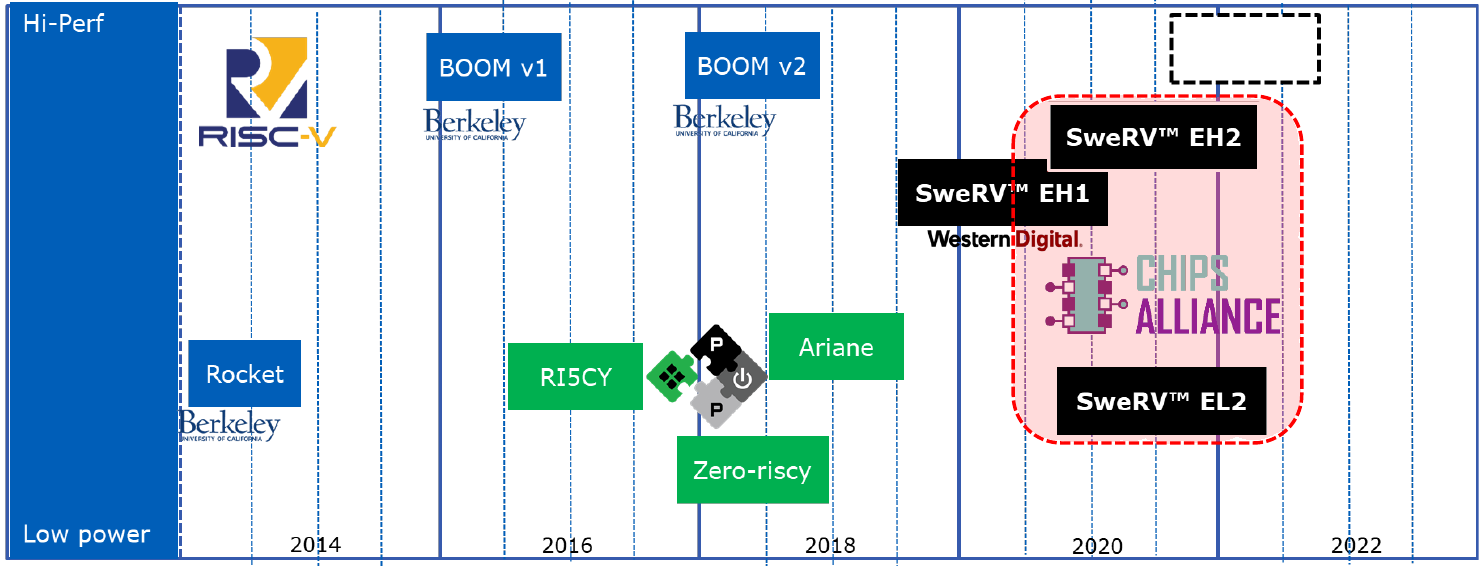
\includegraphics[width=.7\linewidth]{Images/roadmap_compare2.png}
        \caption{Comparativa de la potencia de varios Cores RISC-V de código abierto. Extraído de \citetitle{SweRVRoadmap}~\cite{SweRVRoadmap}.}
        \label{fig:roadmap_compare}
    \end{figure}
    
    \nocite{RepoSwervEL2}
\end{frame}

\begin{frame}{Microarquitectura SweRV-EL2}
        \begin{columns}[t]
            \column{.5\linewidth}
            \begin{figure}[t]
                \centering
                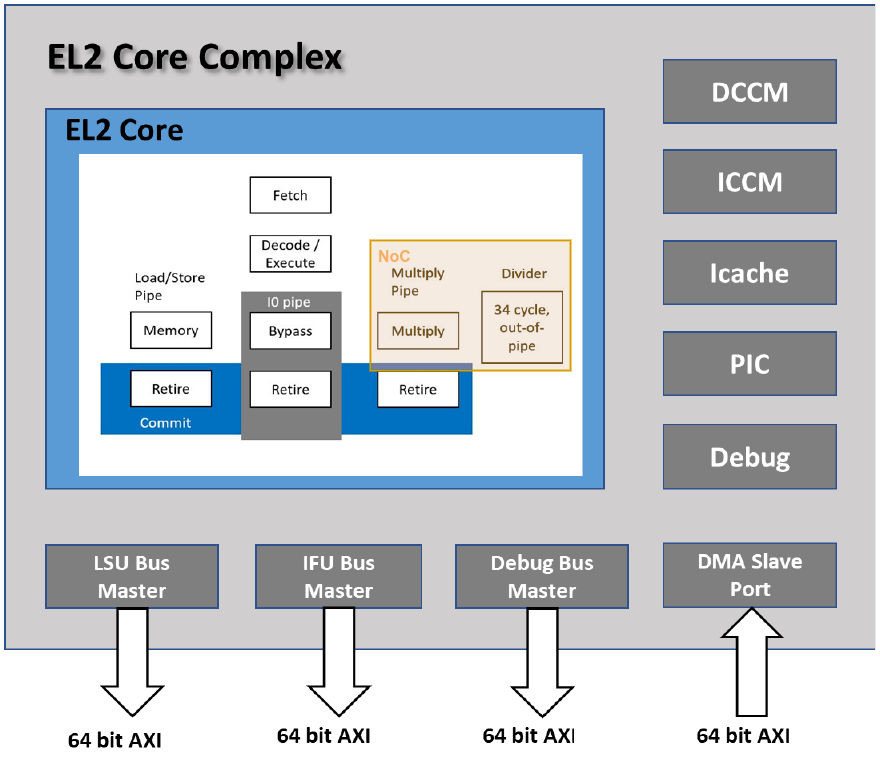
\includegraphics[width=.70\linewidth]{Images/swerv_architecture.drawio2.png}
                \caption{Complejo del SweRV-EL2. Señalado en naranja las partes que hacen uso de la NoC. Extraído de \citetitle{SweRVRoadmap}~\cite{SweRVRoadmap}.}
                \label{fig:swerv_complex}
            \end{figure}%
            \column{.5\linewidth}\pause%
            \begin{figure}[t]
                \centering
                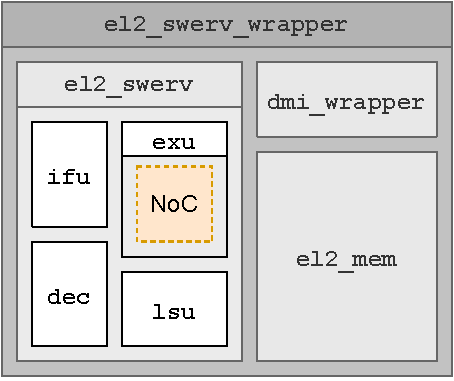
\includegraphics[width=.75\linewidth]{Images/swerv_blocks.drawio.pdf}
                \caption{Diagrama de bloques del procesador modificado.}
                \label{fig:swerv_blocks}
            \end{figure}
        \end{columns}
\end{frame}
